\section{Calorimeter}

\subsection{ECAL}

Calorimetry literally means ``heat measurement.'' The incident particle interacts with the material in the detector to form a shower of particles which are decelerated and absorbed in the detector material to reconstruct the original particle's energy.  
The ATLAS calorimeter is divided into two parts: the electromagnetic calorimeter (ECAL) and the hadronic calorimeter (HCAL).  The ECAL is for electromagnetic interactions and has higher precision than the HCAL which reconstructs the particles interacting by the strong force.   

\subsubsection{Sampling vs. Homogenous Calorimeters}

For an electromagnetic shower to develop, incident electrons (and positrons) will emit a photon through Bremsstrahlung approximately in through a distance characterized by the radiation length
\begin{equation}
X_0=\frac{716.4~{\text{g}} \cdot {\text{cm}}^{-2}  A}{Z(Z+1) \ln{ \frac{ 287 }{ \sqrt{Z} }}}
\label{radiation_length}
\end{equation}
where $A$ is the number of nucleons and $Z$ is the atomic number (number of protons) in the detector material~\cite{Calorimetry1}.
The units of $X_0$ means that dividing by the density gives the actual distance traveled by a particle \cite{Calorimetry2}.
Then the photons will in turn pair-produce electrons and positrons when traveling a distance of $\frac{9}{7} X_0$.  This showering phenomena will continue until the average particle energy decreases to below the critical energy, $E_c=\frac{610~{\text{MeV}}}{Z+1.24}$.
The hadronic showers are characterized by the interaction length, $\lambda = 37.8 A^{0.312} {\text{g}} \cdot {\text{cm}}^{-2}$, the average distance that an incident particle travels before undergoing a nuclear interaction.  

\begin{wrapfigure}{r}{0.5\textwidth}
\centering
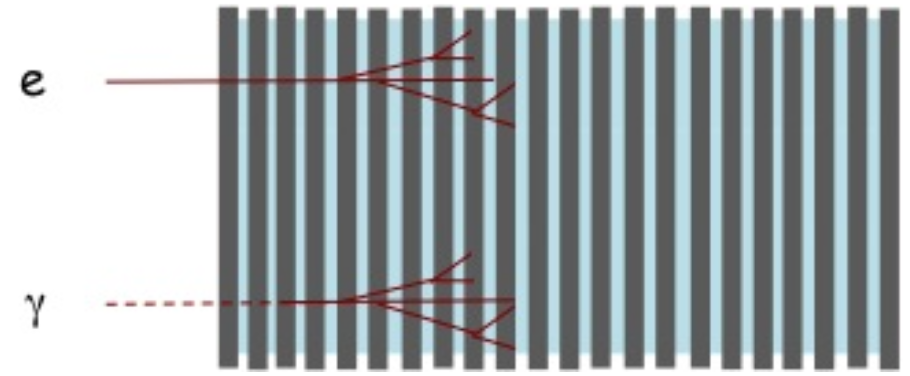
\includegraphics[width=0.45\textwidth]{\figpath/Sampling_Cal.png}
\caption{Schematic illustrating how a sampling calorimeter causes an incident particle to form a shower more quickly.
~\cite{Sampling_Cal}}
\label{sampling-schematic}
%\vspace*{-5mm}
\end{wrapfigure}

Two different calorimeter designs can be used to measure the incident particle's energy.  In a sampling calorimeter, the volume is divided into scattering and absorbing slabs, shown in \Fig{sampling-schematic}.  
The scattering slabs use a high Z material to decrease the radiation length and allow the shower to develop more quickly.  
The energy deposited in the absorbing region of the calorimeter is measured, and the total energy is the energy deposited in the absorbing region divided by a scale factor, $f_{sampling}= E_{visible} / E_{deposited}$.   A sampling calorimeter contains the shower in a smaller detector to help minimize the cost of the experiment.  
One of the downsides of this procedure is that the sampling method is not as precise because only a fraction of the energy deposited is measured, and fluctuations proportional to $\sqrt{E}$ for Poisson statistics will introduce extra errors into the measurements.

A homogenous calorimeter circumvents this problem by using the whole calorimeter as an active volume.  
A homogenous calorimeter is only useful as an ECAL since hadronic interactions require more material to ``contain,'' and it may not be monetarily feasible to construct such a large volume.  
To see this, we can look at the approximate formulas for the radiation length and interaction length, $X_0\sim \frac{A}{Z^2}$ , and $\lambda \sim A^{1/3}$. Since Z is approximately $\frac{1}{2} A$, this means  $\frac{\lambda}{X_0} \sim A^{4/3}$, a number that can be as large as 30 for high Z materials such as lead, showing that hadronic showers have a larger extent.  

\subsubsection{Liquid Argon Detector}
The ATLAS ECAL is a sampling calorimeter arranged in an accordion structure, as shown in \Fig{accordian-structure}.  The high Z material (Z = 82) lead creates the shower, while the energy is measured in liquid argon (LAr), a low Z material (Z = 18).  
As illustrated in \Fig{accordian-structure}, the folding angle decreases as the  radius (measured out from the interaction point) increases.  The folding angle varies between $90^\circ$ and $67^\circ$ to keep the LAr sampling region width approximately constant at 2.1mm between the absorbers.

\begin{figure}[h!tbp]
\centering
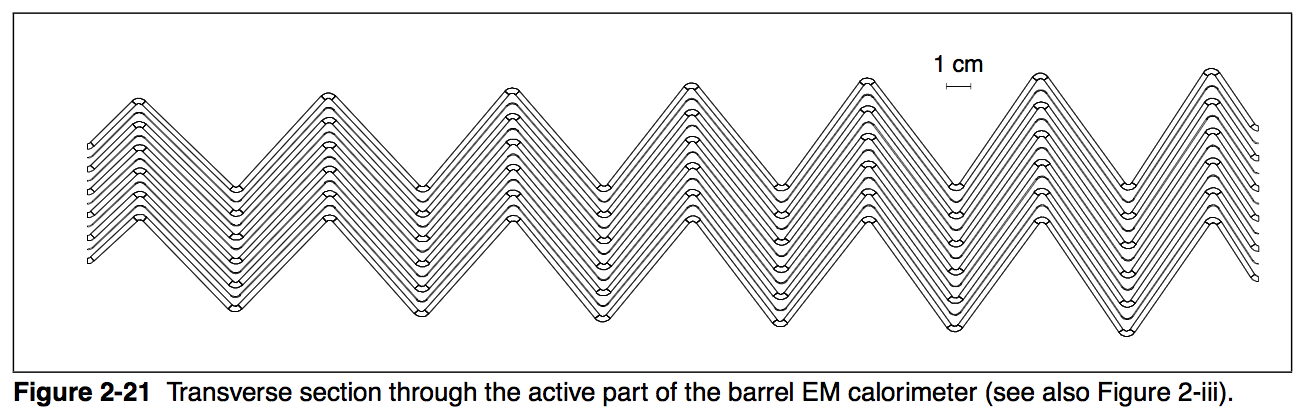
\includegraphics[width=\textwidth]{\figpath/accordian_structure.png}
\caption{Accordian sampling structure for calorimeter.
~\cite{LAr}}
\label{accordian-structure}
\end{figure}

The LAr scintillators are read out with wavelength-shifting photosensors.   
This type of a detector lends itself naturally to a tower structure with the modules forming wedges pointing back to the interaction point, shown in \Fig{Wedge-LAR-accordian}. This makes it easy for a particle's shower to be contained within a few modules or cells.  The segmentation in $\Delta \eta \times \Delta \phi$ is $0.025 \times 0.1$ in the pre-sampler region, $0.0031 \times 0.1$ in the strips, $0.25 \times 0.25$ in the main region, and $0.5 \times 0.025$ in the back region. This yields an energy resolution of 10-12\% GeV$^{-1/2}$.   

\begin{figure}[h!tbp]
\centering
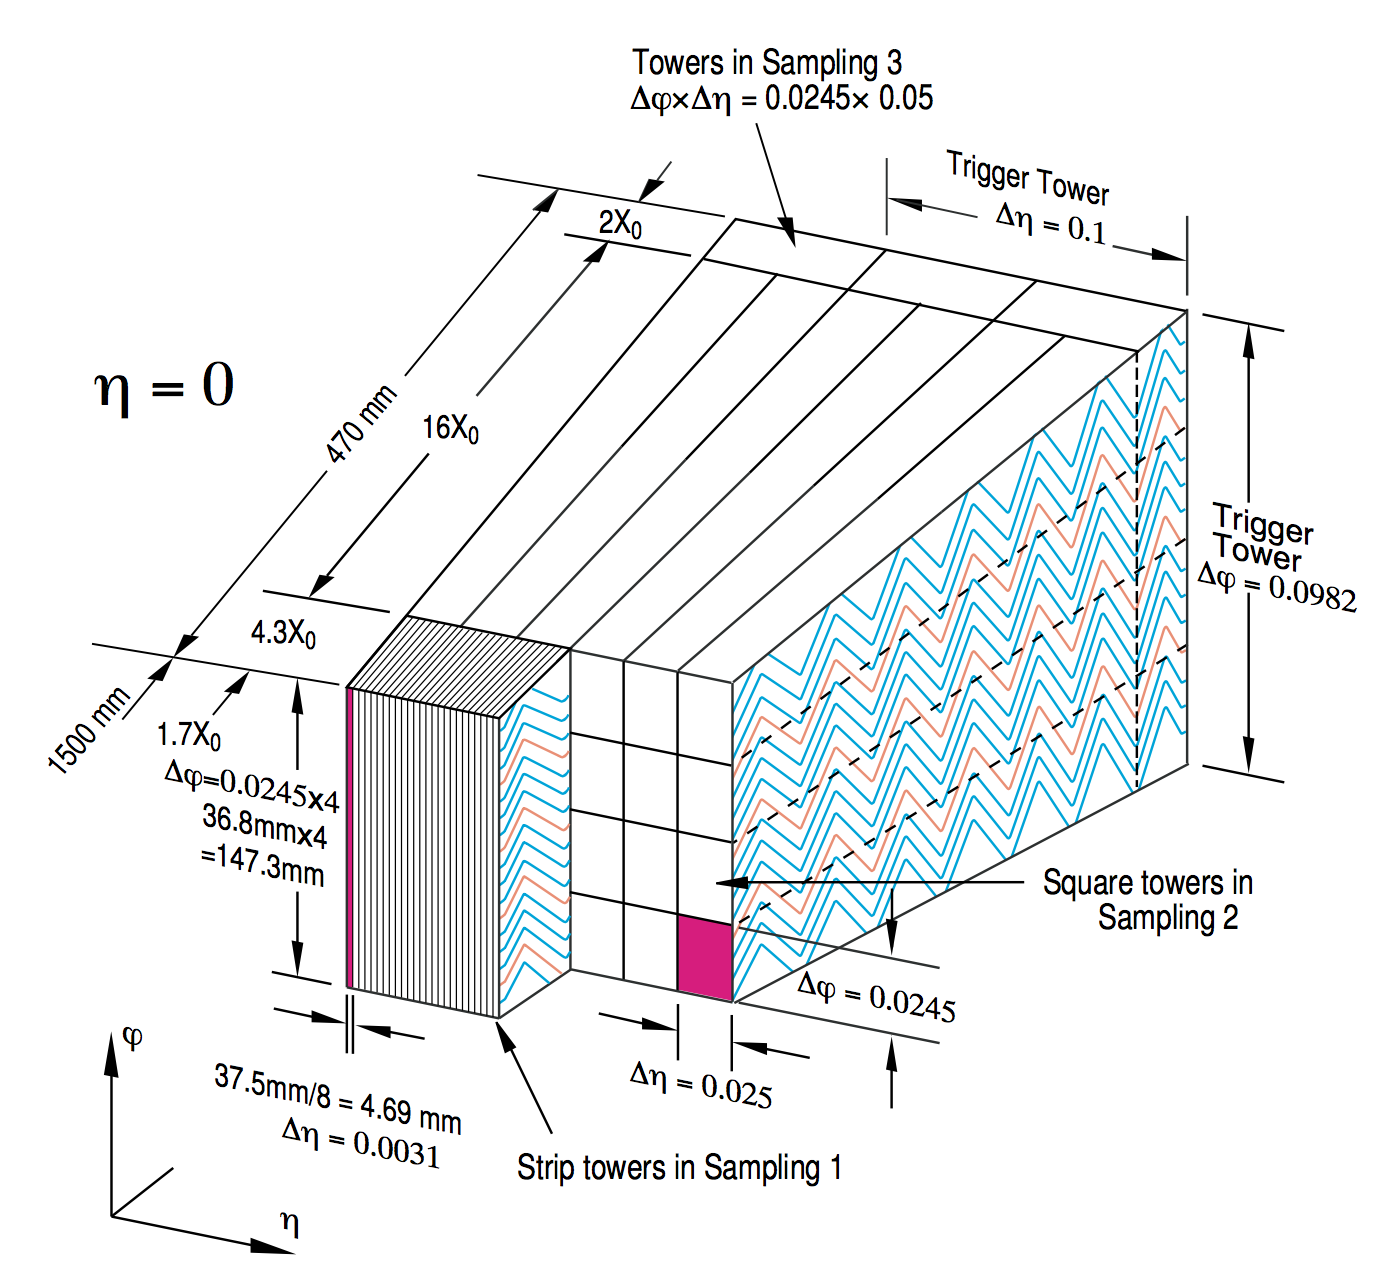
\includegraphics[scale=0.5]{\figpath/Wedge_LAR_accordian.png}
\caption{Wedge showing the accordian structure for the liquid Argon portion of the calorimeter.
~\cite{LAr}}
\label{Wedge_LAR_accordian}
\end{figure}

\subsection{HCAL}

The hadronic calorimeter (HCAL) is the layer just outside of the ECAL, and measures the 
energy of hadrons that traverse the ECAL without stopping, as well as minimum-ionizing particles like muons.
Although the ECAL system could be used to measure the development of the hadronic showers as well, the HCAL system's coarser granularity decreases the monetary cost in covering this larger volume.  It is divided into three parts: the tile calorimeter, the LAr hadronic end--cap calorimeter, and the LAr forward calorimeter, as shown in \Fig{calorimeter}.

\begin{figure}[h!tbp]
\centering
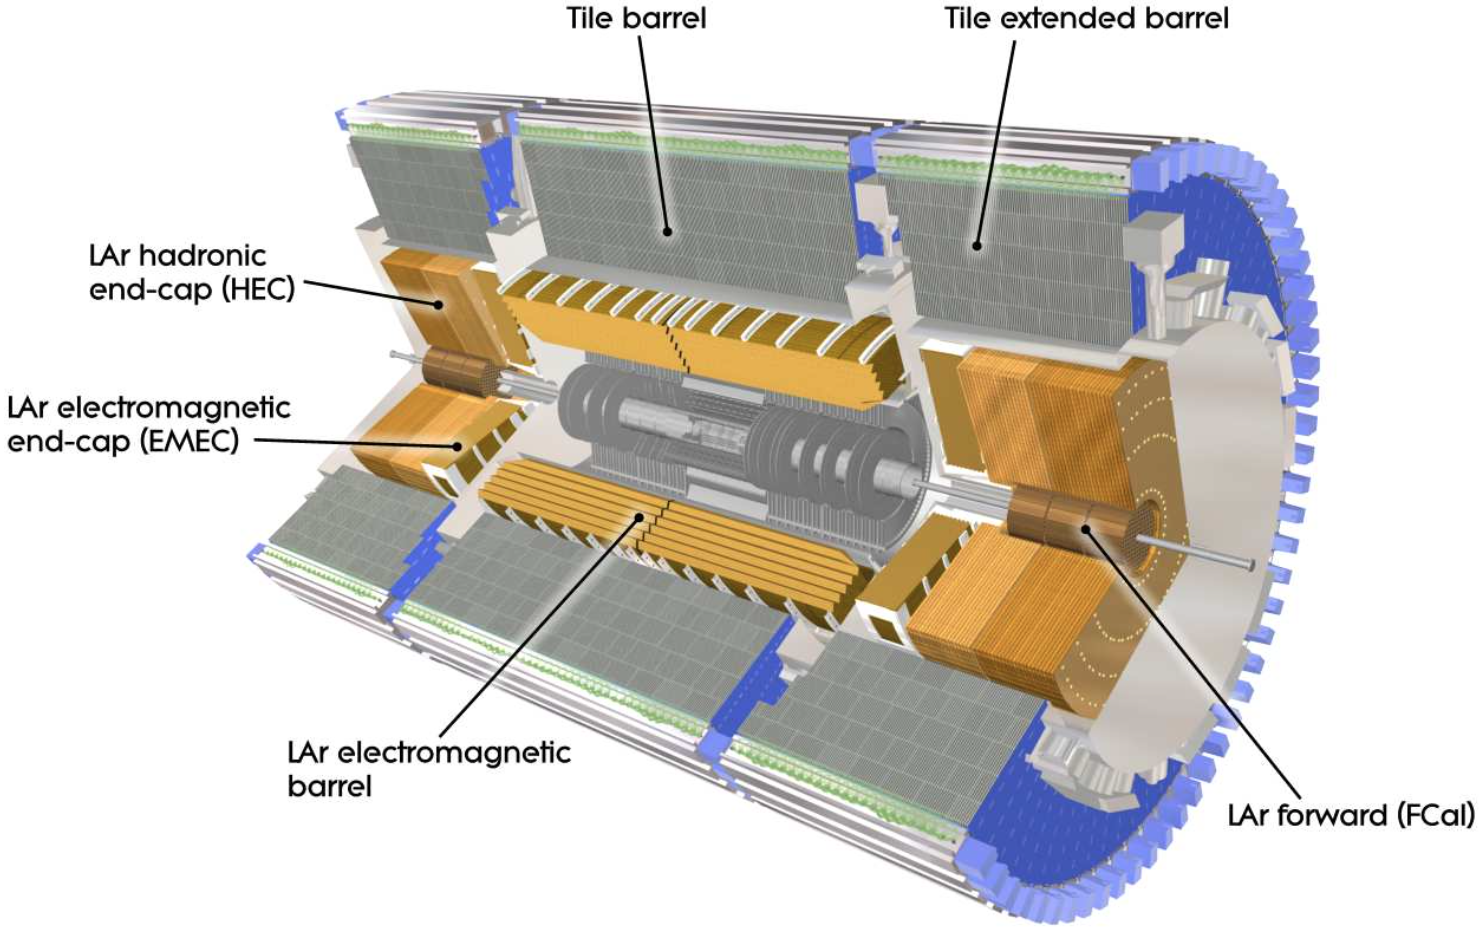
\includegraphics[width=\textwidth]{\figpath/calorimeter.png}
\caption{Calorimeter system at ATLAS~\cite{ATLAS_long}.}
\label{calorimeter}
\end{figure}

\subsubsection{Tile Calorimeter}
The tile calorimeter is just outside ECAL and has an inner radius of 2.28~m and an outer radius 4.45~m.  
The barrel covers $|\eta| < 1.0$, while the extended barrels cover $0.8 < |\eta| < 1.7$.
It is a sampling calorimeter with a steel absorber and scintillating tiles read out with wavelength shifting fibers and photomultiplier tubes. 
Azimuthally divided into 64 modules, the barrel is segmented into three regions at $1.5\lambda, 1.8\lambda$, and $4.25\lambda$, while the extended barrel has $1.5\lambda, 2.6\lambda$, and $3.3\lambda$ depth segmentation.
At $\eta = 0$, the HCAL has a 9.7$\lambda$ depth \cite{ATLAS_long}.

\subsubsection{LAr hadronic end--cap calorimeter}
The LAr hadronic end--cap calorimeter has two wheels per endcap just behind the ECAL endcap calorimeter and housed within the same LAr cryrostats.
The wheels have two depth segments, 25~mm parallel copper plates for the wheels closest to the interaction point, and 50~mm plates for the wheels farther from the interaction point.  The wheels are divided into 32 wedges, with inner and outer radii of 0.475m and 2.03m, respectively.  The copper plates are filled with LAr as the active sampling volume \cite{ATLAS_long}.

\subsubsection{LAr forward calorimeter}
The forward calorimeter covers $\eta >3.1$ and is approximately 10 interaction lengths deep.
Each side has three modules, the first of copper  for electronic measurements, and the second two of tungsten for hadronic measurements.

